\documentclass[twoside]{jsarticle}

\usepackage{grares}
\usepackage[dvipdfmx]{graphicx}
\usepackage{amsmath,amssymb}

\title{ ターボ符号器における決定論インタリーバの設計に関する研究}
\name{Bohulu Kwame Ackah}
\srnum{1631133}
\bib{}
\adviser{橋本 猛{情報伝送研究室}}
\date{}



\begin{document}
\MKTITLE


\section{はじめに }
ターボ符号(TC)は、Claude Berrouさんが開発された高性能な誤り訂正符号であり、AWGNチャネルの場合のシャノン限界に最も近い誤り訂正符号の一つである。ターボ符号二つの再帰的畳み込み符号(RSC符号)をインタリーバで並列連結して作られている。その二つのRSC符号は、要素符号と呼ばれている。
ターボ符号のシステム図は図1に描かれている。
\begin{figure}[h!]
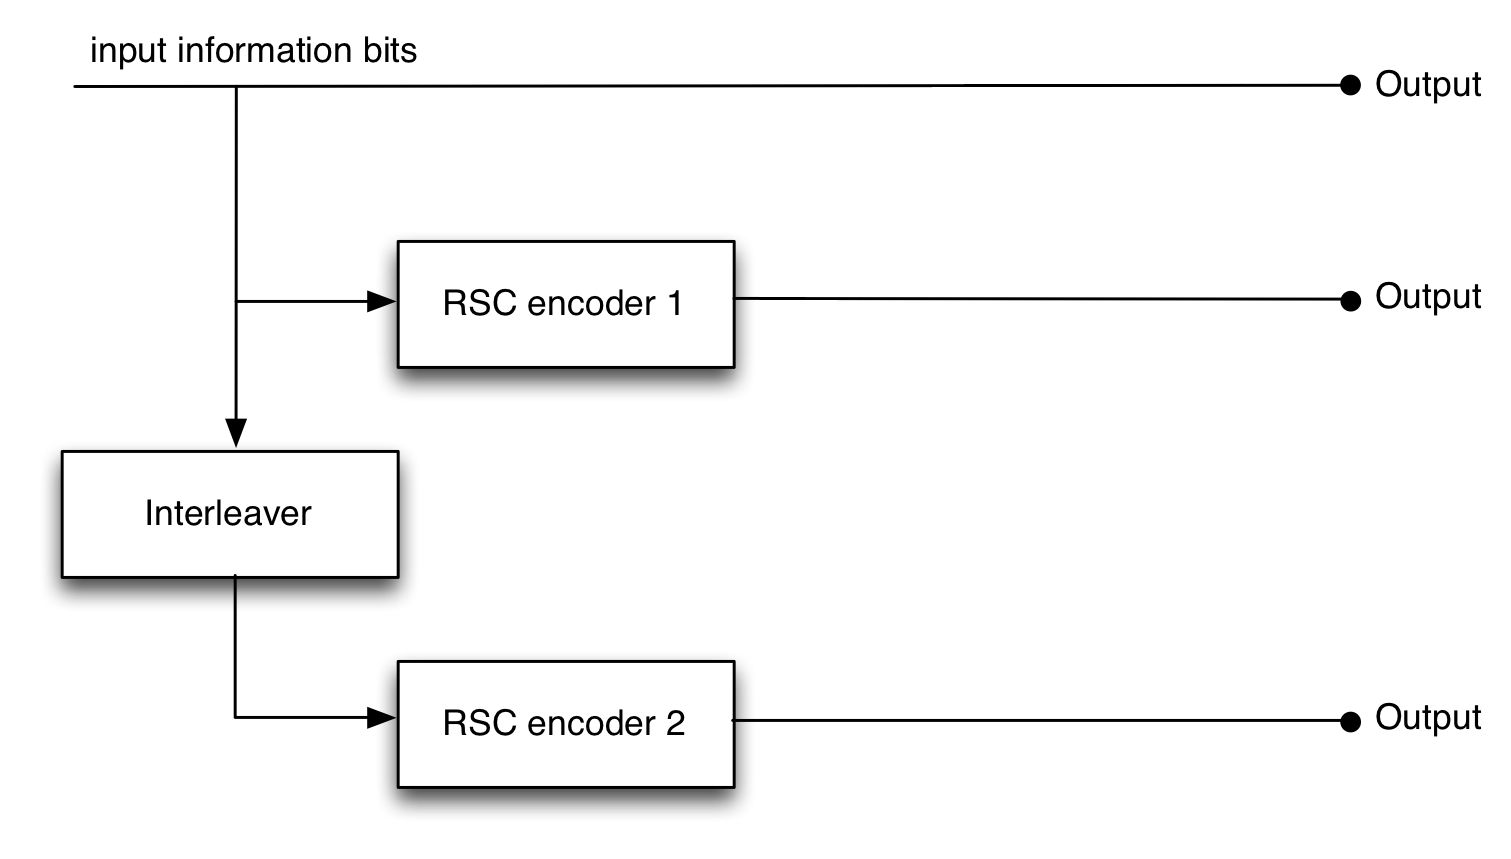
\includegraphics[width=6cm]{TurboEncoderNew.jpg}
\caption{ターボ符号器}
\label{}
\end{figure}
ターボ符号器で使用するインタリーバは、一般的に、ランダムインタリーバと決定論インタリーバの二つのグループにわかれている。ランダムインタリーバは長いフレームサイズの場合、性能が良いですが、ランダムインタリーバを使用するTCは符号器と復号器にインタリーバテーブルを保存しなくてはいけない。応用でたくさんのインタリーバを使用する必要がある場合、ランダムインタリーバは望ましくない。そのかわりに、決定論インタリーバを使用する。インタリーブとデインタリーブはアルゴリズムでできるからである。短いフレームサイズの場合は、決定論インタリーバの性能はランダムインタリーバより良いですが、長いフレームサイズの場合、ランダムインタリーバより良い決定論インタリーバはまだ見つかっていない。%本研究では、長いフレームサイズの場合でも、ランダムインタリーバより良い性能を持つ決定論インタリーバを設計することです。




\section{システムモデル }
シミュレーションで使用するシステムモデルは図1に描かれている。
\begin{figure}[h!]
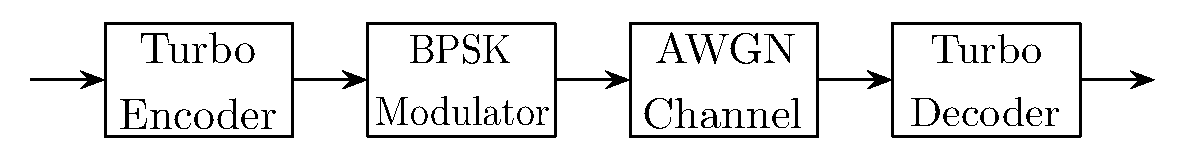
\includegraphics[width=8cm]{figure4.pdf}
\caption{システムモデル}
\label{}
\end{figure}
長さNを持つ情報系列$\mathbf{x}$はターボ符号器の1番目の要素符号(CE1)に入力し、$\mathbf{x}$をインタリーバで並び替えて、2番目の要素符号(CE2)に入力する。CE1とCE2 は同じRSC符号器である。ターボ符号器の出力$\mathbf{y}$は長さを$(n+1)N$を持ち、BPSK変調器の入力である。BPSK変調器はビット''1''を+1に変調し、、ビット''0''を-1に変調する。変調された出力$\mathbf{\widetilde{y}}$はAWGNチャネルで送信され、AWGNチャネルの出力$\mathbf{\widehat{y}}$はターボ符号復号器に入力する。ターボ復号器の出力$\mathbf{\widehat{x}}$は長さNで、$\mathbf{x}$の推計である。
ここで、この資料で使用される記号は,表1にまとめる。


\begin{center}
 \begin{tabular}{||c c||} 
 \hline
 記号 & 意味\\ [0.5ex] 
 \hline\hline
 $x_i$ & i番目の情報ビットの位置  \\ 
 
  $d_{ef}$ &TCの有効自由距離  \\ 
  
   $\tau$ & RSC符号の周期  \\ 
 
 $n$ & 1ビットあたりの出力ビット  \\
 
 $K$ & 要素符号器の拘束長 \\
 
 $R$ & ターボ符号の出力レート \\
 
 $\tau$ &  要素符号器の周期 \\
 
 $t$ & CE1で、タイプ1エラーイベントの長さ\\ 
 
  $s$ & CE2で、タイプ1エラーイベントの長さ\\ [1ex] 
 \hline
\end{tabular}
\end{center}

\section{ターボ符号器の性能解析}
ターボ符号を作るのに、RSC符号は大変重要です。RSC符号は再帰的で、自由距離のプロパティが良いからである。研究で明らかになったのはSNRが高い場合、TCのビット誤り率性能はTCの$d_{ef}$制限されている。$d_{ef}$とは、入力重み2エラーイベントが入力された場合のターボ符号語の最低距離である。入力重み2エラーイベントとは、ビット''1''二つがある情報系列である[3]。

%設計されたインタリーバのマッピング関数は以下のように定義される。
%\begin{equation}
%\Pi(x_i) =[x_iD +\left \lfloor{x_i/A}\right \rfloor ]_N  %\[iD + \lfloor{\frac{i}{A}} \]\rfloor
%\end{equation}
%$$1 \leq D \leq L, C:=gcd(N,D), A:=N/C$$
%設計されたインタリーバを使用するターボ符号のビット誤り率性能を試さなくてはいけない。
最尤復号とAWGN チャネルの場合、畳み込み符号のビット誤り率性能はupper bound technique上界できる[2]。


\begin{equation}
P_b \leq \sum_{i=1}^{2^N} \frac{w_i}{N}Q\Bigg( \sqrt{d_i\frac{2RE_b}{N_o}}\Bigg)
\end{equation}
 $w_i$ と $d_i$は$i$番目の符号語の組織ビットの重みと合計ハミング重みである。ターボ符号は畳み込み符号から作られているので、(2)でターボ符号のビット誤り率性能の上界が計算できる。TCに関する重み2エラーイベントの合計出力重みは以下の式で計算できる[3]
\begin{equation}
d_{(t,s)}=6+\Bigg( \frac{ \left|t\right|}{\tau} + \frac{ \left|s\right|}{\tau} \Bigg)w_o
\end{equation}
$w_o$は$1+D^\tau$の形を持つ入力系列の場合、一番目の要素符号の出力の重みである。目的は$t+s$の最低値を大きくする$D$見つけることである。

$t$と$s$のすべての可能な値で、(2)で計算された同じ合計ハミング重みを持つ符号語が集められ、符号語あたりの平均組織ビット重みは以下のように定義する[1]。
$W_d$は重み$d$を持つ符号語の合計組織ビットの重みで、 $N_d$は重み$d$を持つ符号語の数である。それで、(2)を以下のように書き換えられる。


\begin{equation}
P_b \approx \sum_{i=1}^{l} \frac{2N_d}{N}Q\Bigg( \sqrt{d_{(t_i,s_i)}\frac{2RE_b}{N_o}}\Bigg)
\end{equation}
$l$は整数組$(t,s)$の合計数である。

$$l=\sum_{a=1}^{3}N-(N-a\tau)$$





\section{インタリーバ設計方法}
代表的な重み2mエラーイベントは図2に描かれている。$m=1,2,...$ターボ符号にある重み2エラーイベントはそれぞれの要素符号にあるm個の重み2エラーイベントのことでありインタリーバで繋がっている。
\begin{figure}[h!]
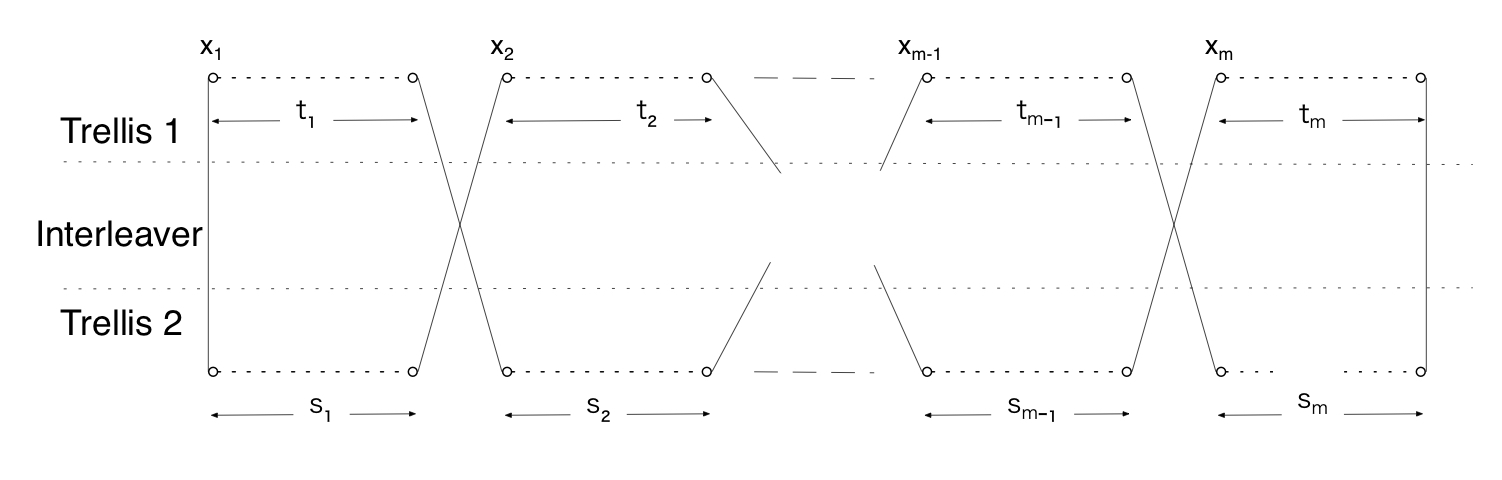
\includegraphics[width=8cm]{weight2m.jpg}
\caption{代表的な入力重み2mエラーイベント}
\label{}
\end{figure}
CE1でのi番目の重み2mエラーイベントは長さ$t_i$を持ち、$x_i$から$x_i+t_i$まである。\\$$x_i \in \mathbb{Z},  t_i \in \tau \cdot \mathbb{Z} \triangleq \mathbb{D}$$エラーイベントの開始と終了は$(x_i,x_i+t_i)$の整数組で表現されている。CE2でのi番目の重み2エラーイベントは長さ$s_i$で、エラーイベントの開始と終了は$(x_i,x_i+s_i)$の整数組で表現されている。

基本の場合$m=1$に注目すると、以下の図を使用してインタリーバの設計をする。
\begin{figure}[h!]
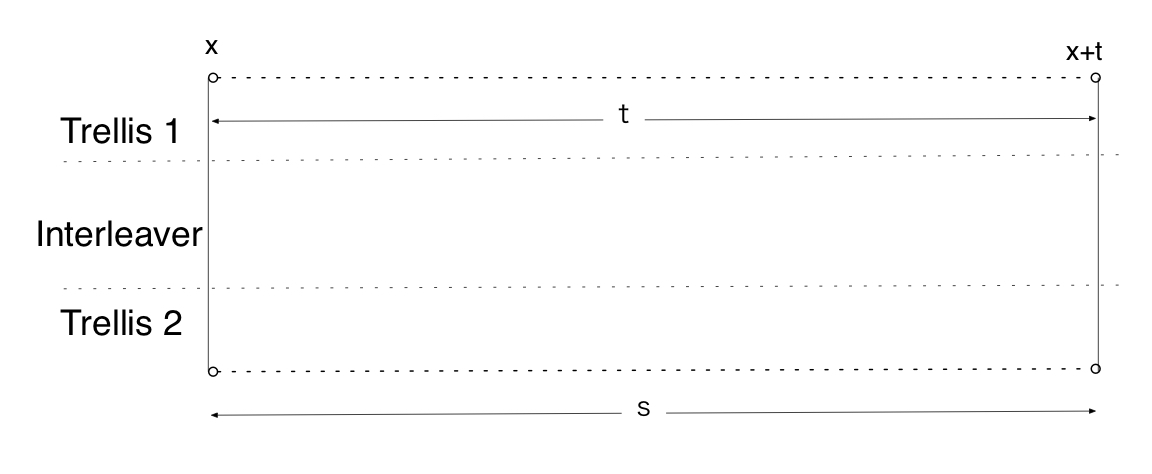
\includegraphics[width=8cm]{weight2.jpg}
\caption{入力重み2エラーイベント}
\label{}
\end{figure}
研究で明らかになったことは、$(1+D^{a\tau})(D^u) ,0\leq u\leq N-\tau$の形を持つ入力重み2エラーイベント(タイプ1エラーイベント)はRSC符号に入力する場合低い重みをもつ符号語を作成する。ターボ符号の$d_{ef}$を大きくするために$$s \leq a\tau \triangleq \mathbb{E}(s) \\\\\ \forall x \in \mathbb{Z} , t \in \mathbb{D}$$の場合を防ぐようなインタリーバを設計したい、特に最悪の場合の$t = s =\tau$である。言い換えると、ターボ符号の$d_{ef}$値を大きくするために、可能な限り$t+s$を大きくしたいである。






\section{Dの検索方法}

\begin{thebibliography}{}
  \bibitem{1}  Oscar Y. Takeshita, Member, IEEE, and Daniel J. Costello ,''New Deterministic Interleaver Designs for Turbo Codes'',IEEE Trans. Inform. Theory, vol. 46,pp. 1988-2006,Nov. 2000\\
  \bibitem{2} L. C. Perez, J. Seghers, D. J. Costello, Jr., ''A distance spectrum interpretation of turbo codes'', IEEE Trans. Inform. Theory, vol. 42, pp. 1698-1709, Nov. 1996.\\
\bibitem{3} Jing Sun, Oscar Y. Takeshita ”Interleavers for Turbo Codes Using Permutation Polynomials over Integer Rings”, IEEE Trans. Inform. Theory, vol. 51,
pp. 101 - 119 Jan. 2005\\
\bibitem{4} John G. Proakis, Masoud Salehi. ''Digital Communications'', Fifth Edition,Chapter 8, McGraw-Hill\\.
\end{thebibliography}



\end{document}
